\chapter{研究假設與架構}
\section{概念架構}
本研究根據文獻探討的回顧與整理,建立研究之架構如圖:\ref{fig:ARC}所以示本研究探討品牌知覺與品牌聲望與網路消費者決策和消費者滿意度之間的關係,暸解品牌聲望與品牌知覺對網路消費者決策與網路消費者滿意度之研究,並建立本研究架構。


\begin{figure}[h]
\centering
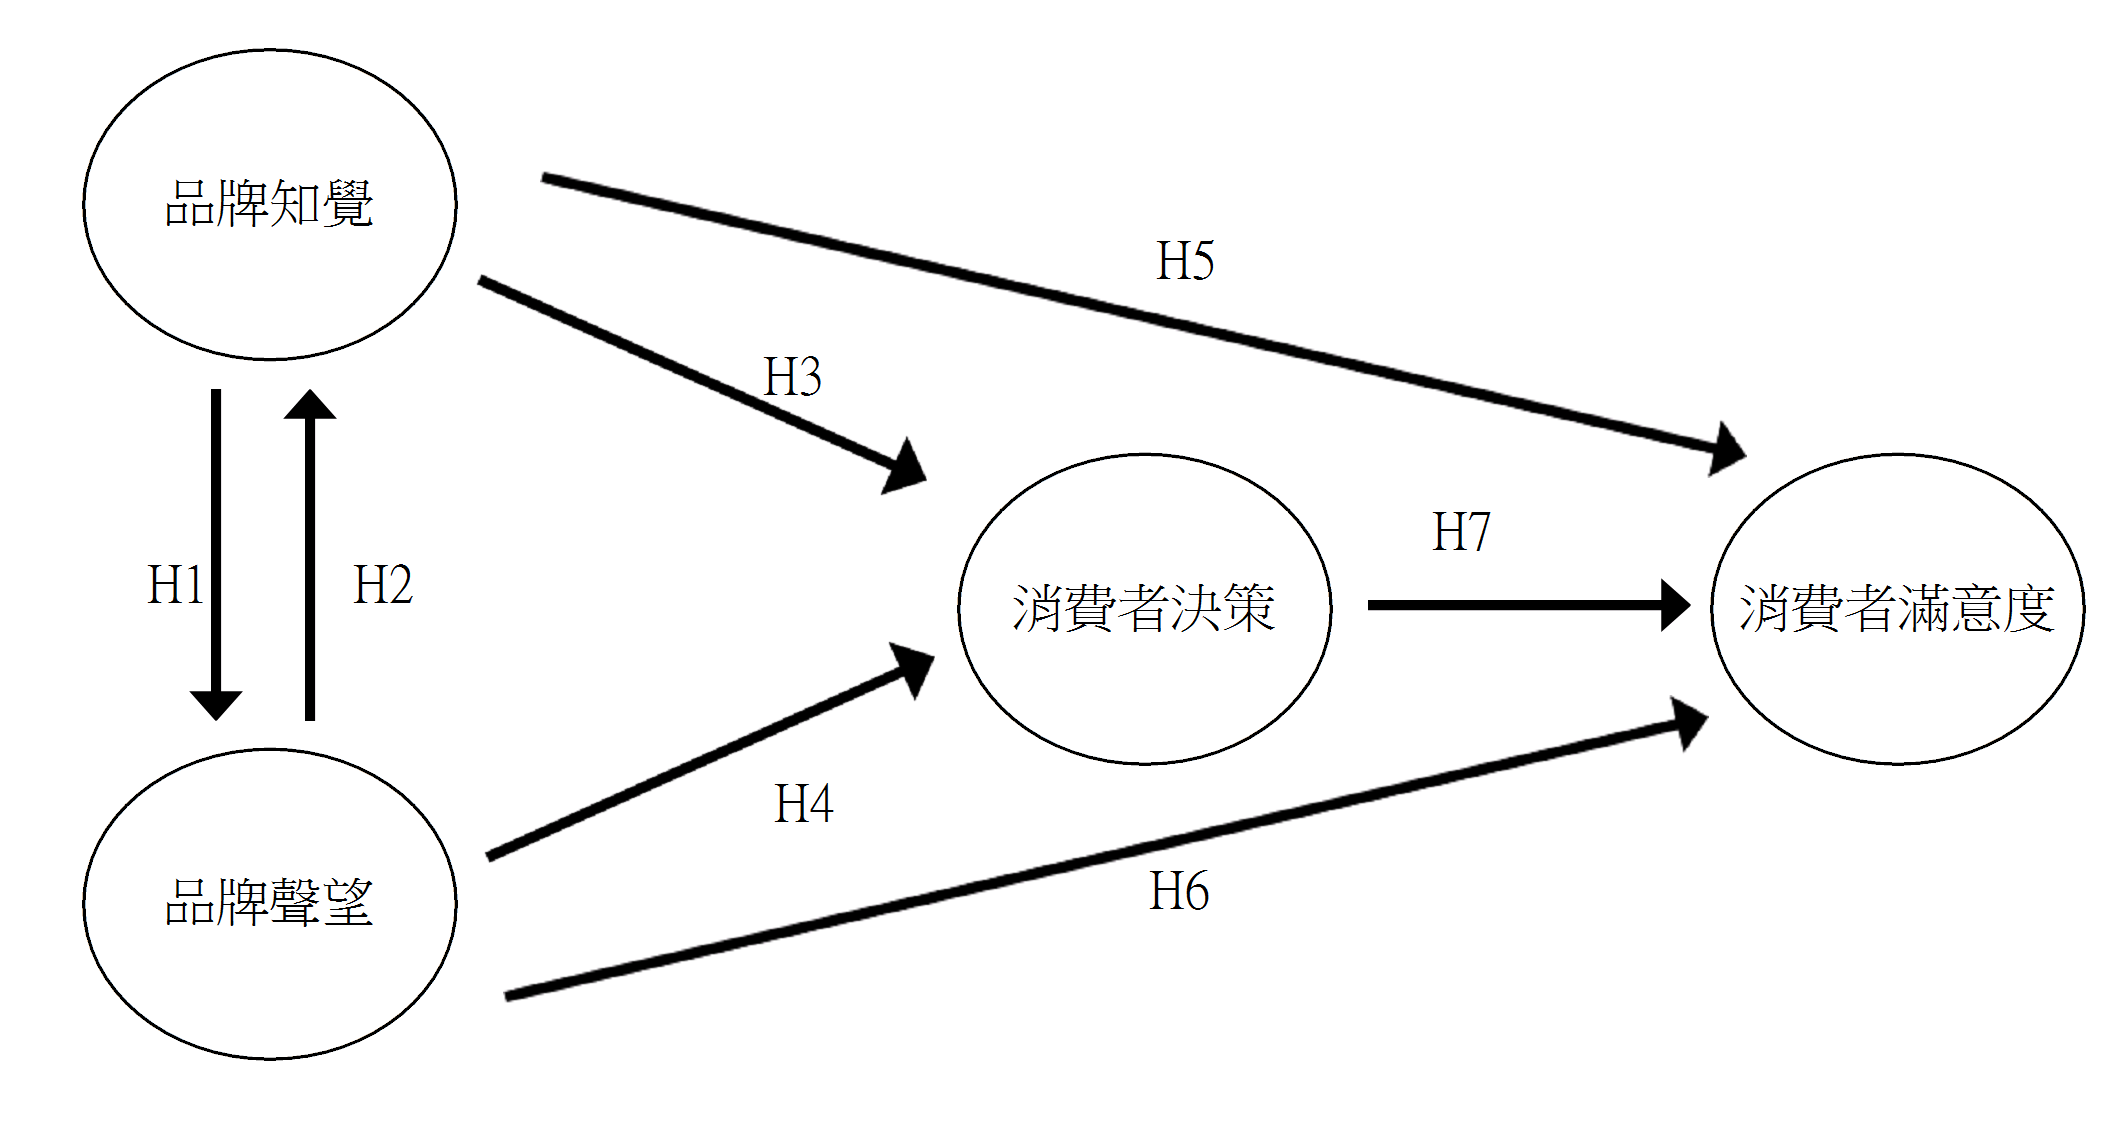
\includegraphics[width=14cm]{images/論文架構.png}
\caption{研究架構}
\label{fig:ARC}
\end{figure}

\section{研究假設}
根據上述的的目的,本研究嘗試提出以 下假設:
\begin{enumerate}
\item 根據Aaker (1991) 將消費者對品牌的知覺品質定義為消費者對於某一 項品牌產品整體品質的認為水準,或消費者對在特定目的下相對於其他品牌, 對某品牌產品或服務全面品質的主觀滿意程度,基於以上的推論,本研究提出以下的研究假設 :

H1品牌知覺會正向影響品牌聲望有顯著的關係

H2品牌聲望會正向影響品牌知覺有顯著的關係

\item 根據 Rao and Ruekert (1994) 品牌對於消費者而言是屬於產品的一部分,可視為傳遞產品品質訊息的媒介,而且往往是消費者購買決策的重要考量因素之一,基於以上的推論,本研究提出以下的研究假設 :

H3品牌知覺會正向影響消費者決策有顯著的關係

H4品牌聲望會正向影響消費者決策有顯著的關係

\item 根據藍悅真(2012)指出品牌會影響消費者滿意度,Oliver (1980) 指出消費者如之前購買經驗是否感到滿意,而決定是否再次購買;基於以上的推論,本研究提出以下的研究假設 :

H5品牌知覺會正向影響消費者滿意度有顯著的關係

H6品牌聲望會正向影響消費者滿意度有顯著的關係

H7消費者決策會正向影響消費者滿意度有顯著的關係

\end{enumerate}

\section{研究對象與抽樣方法}
本研究目的主要探討品牌知覺,品牌聲望對消費者決策與消費者滿意度之關係,並提出對公司意見與建議,以網路使用者為受訪為樣本,問卷蒐集方式採用Google Docs「網路問卷調查表」以網路散播方式發放。

本研究共有五大部份,第一部分蒐集樣本的性別、年齡等人口統計變數資料,後前四部分均以李克特(Lilert)五點尺度量表來 衡量(1=非常不同意,2=不同意,3=不同意也非不同意,4=同意,5=非常同意)。
第二部分衡量消費者決策共10題,第三部分衡量品牌知覺共有8題,第四部分衡量品牌聲望共有10題,第五部分衡量消費者滿意度共有10題

\section{變數的定義與衡量}
\begin{enumerate}
\item  網路消費者決策共有10個題目在網路上選購精品、珠寶商品時會參考的因素:價錢、品牌形象、製造材料與特性、其他顧客反應度、商品認證保證、售後服務、交貨服務、整體商品的價值、品牌知名度、設計感
\item 品牌知覺共有7個題目知覺對鈦鍺的所產生出來的狀況:商品的品質良好、鈦鍺品牌形象、製作材料(與特性)、商品外觀設計很滿意、商品的廣告或名稱很滿意、整體商品的價值、品牌知名度
\item 品牌聲望共有10個題目得到相關資訊是否有幫助您了解LaJolla鈦鍺精品:價錢、品牌形象、製作材料(與特性)、其他顧客反應、商品認證保證、售後服務、交貨服務、整體商品的價值、品牌知名度、設計感
\item 消費者滿意度共有10題目購買相關LaJolla鈦鍺精品的滿意度:價錢、品牌形象、製作材料(與特性)、其他顧客反應、商品認證保證、售後服務、交貨服務、整體商品的價值、品牌知名度、設計感
\end{enumerate}

\section{資料分析方法}
本研究利用統計分析套件軟體 SPSS 20進行相關分析,使用的分析如下
\begin{enumerate}
\item 描述性統計 :分析樣本結構中性別,年紀教育,程度工作性質的百分比
\item 信度分析:以Cronbach's 值來鑑定各量表的內部一致性
\item 因素分析:主要目的將原有很多變數(維度)之資料,縮減成較少的維度數,但有保持原本所提供的資料
\item 簡單迴歸:分析進行假設的驗證
\end{enumerate}

本研究探討品牌知覺、品牌聲望、消費者滿意度之間的關係。本研究已發放問卷的方式取的資料,問卷填寫主要以網路發放題目主要
品牌知覺、品牌聲望、消費者滿意度以簡單迴歸分析來驗證假設是否成立

\chapter{研究結果展示}
\section{敘述統計}
本研究採用網路與百貨公司附近發放方式,針對可能聽過鈦鍺精品的人進行問卷調查供調查603份剔除重複填寫與漏填,有效問卷599份 
本研究的樣本資料分析結果顯示 
\begin{enumerate}
\item 男性佔 50.4 % 女性 49.6% 如表 \ref{tab:PL1} 所示 
\item 年齡分為18歲以下 9.7% 、19 ~25歲 72.0% 、26~35歲 9.8%、36~40歲2.7% 、40歲以上5.8%本問卷族群與年輕族群居多。如表  \ref{tab:PL2} 所示
\item 教育方面 高中以下4.1%、高中(職)19.2%、專科5.3%、大學63.7%、碩士5.3%、博士1.7% 教育程度以大學64.7%為最多 。如表 \ref{tab:PL3} 所示
\item 工作性質 學生52.8%、服務業29.5%、製造業3.5%、軍公教4.3%、自由業8.5%、管家1.3%由職業可看以學生64.7%為最高。如表 \ref{tab:PL4} 所示
\end{enumerate}

\begin{table}[htb]
\caption{敘述統計(性別)}
\label{tab:PL1}
\renewcommand{\arraystretch}{1.2} % 將表格行間距加大為原來的 1.2 倍
\arrayrulewidth=1pt               % 調整線條粗細為 1pt
\tabcolsep=60pt                   % 調整欄間距為 24pt
%\begin{document}
\begin{tabular}[t]{lll}  % 第一欄位使用 sans serif 字族
\hline
 性別&次數 & 百分比 \\
\hline
男生        & 302 & 50.4 \\
女生        & 297  & 49.6 \\
總和        & 599  & 100 \\
\hline
\centering
\label{fig:PL4}
\end{tabular}
\end{table}

\begin{table}[htb]
\caption{敘述統計(年齡)}
\label{tab:PL2}
\renewcommand{\arraystretch}{1.2} % 將表格行間距加大為原來的 1.2 倍
\arrayrulewidth=1pt               % 調整線條粗細為 1pt
\tabcolsep=60pt                   % 調整欄間距為 24pt
%\begin{document}
\begin{tabular}[t]{lll}  % 第一欄位使用 sans serif 字族
\hline
 年齡& 次數 & 百分比 \\
\hline
18歲以下        & 58  & 9.7 \\
19~25歲        & 431  & 72.0 \\
26~35歲        & 59  & 9.8 \\
36~40歲        & 16  &2.7\\
40歲以上        & 35  & 5.8 \\
總和               & 599  & 100 \\
\hline
\end{tabular}
\end{table}

\begin{table}[htb]
\caption{敘述統計(學歷)}
\label{tab:PL3}
\renewcommand{\arraystretch}{1.2} % 將表格行間距加大為原來的 1.2 倍
\arrayrulewidth=1pt               % 調整線條粗細為 1pt
\tabcolsep=60pt                   % 調整欄間距為 24pt
%\begin{document}
\begin{tabular}[t]{lll}  % 第一欄位使用 sans serif 字族
\hline
 學歷& 次數 & 百分比 \\
\hline
高職以下       & 25  & 4.2 \\
高中(職)        & 116  &19.4\\
專科        & 32  & 5.3 \\
大學        & 384 &64.1\\
碩士        & 32  & 5.3 \\
博士           & 10  & 1.7 \\
總和           & 599  & 100 \\
\hline
\end{tabular}
\end{table}

\begin{table}[htb]
\caption{敘述統計(工作性質)}
\label{tab:PL4}
\renewcommand{\arraystretch}{1.2} % 將表格行間距加大為原來的 1.2 倍
\arrayrulewidth=1pt               % 調整線條粗細為 1pt
\tabcolsep=60pt                   % 調整欄間距為 24pt
\begin{tabular}[t]{lll}  % 第一欄位使用 sans serif 字族
\hline
 工作性質& 次數 & 百分比 \\
\hline
學生           & 316  & 52.8 \\
服務業        & 177  & 29.5 \\
製造業        & 21  & 3.5 \\
軍公教        & 26  &4.3\\
自由業        & 51  & 8.5 \\
家管           & 8  & 1.3 \\
總和               & 599  & 100 \\
\hline
\end{tabular}
\end{table}

\section{信度分析}
首先對樣本收集已說明,其次對本研究的變數衡量做信度分析最後驗證假設
信度分析:已進行實證分析針對問卷問項進行信度分析用來得知問卷設計所測得的結果是否有信度與穩定性本研究採用目前已研究最常使用的 信賴度數做信度量測指標 Nunnally(1978)認為信度0.7以上表示高信度 可接受值大於0.7

本研究共有 3個變數,信度分析結果顯示
\begin{enumerate}
\item 消費者決策Cronbach's Alpha 值 0.946  如表 \ref{tab:e1}  所示
\item 品牌知覺Cronbach's Alpha 值 0.936  如表 \ref{tab:e2}  所示
\item 品牌聲望Cronbach's Alpha 值  0.958 如表 \ref{tab:e3}  所示
\item 消費者滿意度Cronbach's Alpha 值 0.969 如表 \ref{tab:e4}  所示
\end{enumerate}
以上信度 Alpha 值 大於 0.7以上顯示本研究的變數具有不錯的可信度。

\begin{table}[htb]
\caption{信度 (消費者決策)}
\label{tab:e1}
\renewcommand{\arraystretch}{1.2} % 將表格行間距加大為原來的 1.2 倍
\arrayrulewidth=1pt               % 調整線條粗細為 1pt
\tabcolsep=18pt                   % 調整欄間距為 24pt
\begin{tabular}[t]{lllll}  % 第一欄位使用 sans serif 字族
\hline
  & 代號& 平均數 & 標準差&  Alpha 值  \\
\hline
消費者決策&決策1&3.9873&0.82930&0.945735\\
               &決策2&3.9429	&0.82742&\\	
               &決策3&3.9460&0.81796&\\
               &決策4&3.9143&0.85713&\\
               &決策5&4.0540&0.82955&\\
               &決策6&4.0476&0.84515&\\
               &決策7&3.9905&0.83508&\\
               &決策8&4.0413&0.83792&\\
               &決策9&3.8381&0.86094&\\
               &決策10&3.9905&0.86136&\\
\hline
\end{tabular}
\end{table}

\begin{table}[htb]
\caption{信度 (品牌知覺)}
\label{tab:e2}
\renewcommand{\arraystretch}{1.2} % 將表格行間距加大為原來的 1.2 倍
\arrayrulewidth=1pt               % 調整線條粗細為 1pt
\tabcolsep=18pt                   % 調整欄間距為 24pt
\begin{tabular}[t]{lllll}  % 第一欄位使用 sans serif 字族
\hline
 & 代號& 平均數 & 標準差&  Alpha 值  \\
\hline
品牌知覺 & 知覺1  & 3.7753   & 0.7479  &0.936242 \\
              & 知覺2  & 3.7483  &0.79497  &  \\
             & 知覺3  & 3.8345    & 0.80373  &  \\
             & 知覺4 & 3.7500   &0.75513  &\\
             & 知覺5   & 3.7534  & 0.77393 &  \\
             & 知覺6  & 3.7534    &  0.77393 & \\
             & 知覺7  & 3.6909     & 0.80231  &  \\
\hline
\end{tabular}
\end{table}


\begin{table}[htb]
\caption{信度 (品牌聲望)}
\label{tab:e3}
\renewcommand{\arraystretch}{1.2} % 將表格行間距加大為原來的 1.2 倍
\arrayrulewidth=1pt               % 調整線條粗細為 1pt
\tabcolsep=18pt                   % 調整欄間距為 24pt
\begin{tabular}[t]{lllll}  % 第一欄位使用 sans serif 字族
\hline
 & 代號& 平均數 & 標準差&  Alpha 值  \\
\hline
品牌知覺 & 聲望1  & 3.6835 &0.82500 &0.958532\\
              & 聲望2  & 3.7089 &0.83439 &  \\
             & 聲望3  &3.6962 &0.85266  &  \\
             & 聲望4  &3.5949&0.75987\\
             & 聲望5  & 3.7468 &0.83924 &  \\
             & 聲望6  & 3.6456&0.78508& \\
             & 聲望7  & 3.6709&0.77900  &  \\
             & 聲望8  & 3.7215&0.84636&  \\
             & 聲望9  &3.6456&0.81709&  \\
             & 聲望10  & 3.7848&0.82696 &  \\
\hline
\end{tabular}
\end{table}

\begin{table}[htb]
\caption{信度 (消費者滿意度)}
\label{tab:e4}
\renewcommand{\arraystretch}{1.2} % 將表格行間距加大為原來的 1.2 倍
\arrayrulewidth=1pt               % 調整線條粗細為 1pt
\tabcolsep=18pt                   % 調整欄間距為 24pt
\begin{tabular}[t]{lllll}  % 第一欄位使用 sans serif 字族
\hline
 & 代號& 平均數 & 標準差&  Alpha 值  \\
\hline
品牌知覺 & 滿意度1&3.233&0.97143&0.969024\\
              & 滿意度2&3.4667&1.10589&  \\
             & 滿意度3&3.5000&1.00858&  \\
             & 滿意度4&3.5667&1.13512&\\
             & 滿意度5&3.7000&1.08755&  \\
             & 滿意度6&3.5667&1.16511&\\
             & 滿意度7&3.4667&1.00801&  \\
             & 滿意度8&3.6333&0.99943&  \\
             & 滿意度9&3.4333&1.04000&\\
             & 滿意度10&3.5667&1.07265&\\
\hline
\end{tabular}
\end{table}

\section{因素分析}
為了探討受訪者對主要考量因素,因此提出10提消費者行為、8題品牌知覺、10題品牌知覺、10題消費者滿意度等變數以量表收集受訪者對每一變數之重視度(非常不同意=1、非常同意=5)。將所獲得之資料,經過KMO取樣適當性及巴氏球形檢定,KMO值越高表示進行因素分析的效果越好,其值在0.9以上表示效果極佳,0.8以上表示是有價值的,0.7以上是中度的,0.6以上是不好也不壞,0.5以上是不太好,若值在0.5以下,就表示其效果是無法接受的
\begin{enumerate}
\item 消費者決策
KMO=0.948 大於0.9表示分析效果極佳 Bartlett 的球形檢值 2427.156 顯著性.000<α = 0.01 顯示資料非常適合因素分析  本部分特性值大於1之標準將10個變數濃縮為1個因變數(主成分)全部變異可解釋為67.400%,詳細的數據如表  \ref{tab:p4} 所示。
\item 品牌知覺
KMO=0.926 大於0.9表示分析效果極佳 Bartlett 的球形檢值 3210.519 顯著性.000<α = 0.01 顯示資料非常適合因素分析  本部分特性值大於1之標準將7個變數濃縮為1個因變數(主成分)全部變異可解釋為72.457%,詳細的數據如表  \ref{tab:p4} 所示。
\item 品牌聲望
KMO=0.899 大於0.8表示分析有價值 Bartlett 的球形檢值 800.032 顯著性.000<α= 0.01 顯示資料有價值因素分析  本部分特性值大於1之標準將10個變數濃縮為1個因變數(主成分)全部變異可解釋為73.020% 如圖 \ref{tab:p4}  所示。
\item 消費者滿意度
KMO=0.788 大於0.7表示分析中等 Bartlett 的球形檢值 420.646 顯著性.000<α=0.01 顯示資料中度合因素分析  本部分特性值大於1之標準將10個變數濃縮為1個因變數(主成分)全部變異可解釋為78.632% 如圖 \ref{tab:p4} 所示
\end{enumerate}

\begin{table}[htb]
\caption{因數分析}
\label{tab:p4}
\renewcommand{\arraystretch}{1.2} % 將表格行間距加大為原來的 1.2 倍
\arrayrulewidth=1pt               % 調整線條粗細為 1pt
\tabcolsep=16pt                   % 調整欄間距為 24pt
\begin{tabular}[t]{lllll}  % 第一欄位使用 sans serif 字族
\hline
 項目& KMO值 & KMO值接受度& 巴氏球型檢定&顯著性 \\
\hline
消費者決策&0.948&效果極佳&2427.156&0.000\\
 品牌知覺&0.926&效果極佳&3210.519&0.000\\
 品牌聲望&0.899&有價值&800.032&0.000 \\
消費者滿意度&0.788&中度&420.646&0.000\\
\hline
\end{tabular}
\end{table}

%\begin{figure}[!t]
%\centering
%\includegraphics[width=8cm]{images/kom.PNG}
%\caption{因素分析}
%\label{fig:p4}
%\end{figure}
\section{假設之驗證}
本研究共有6個假設待驗證,均採用簡單迴歸分析,結果整理於表 \ref{tab:HRR} 所示以下對每個假設驗證結果加以說明
\begin{enumerate}
\item 假設1:品牌知覺會正向影響品牌聲望有顯著的關係。
依簡單迴歸分析得值為:依變數[品牌知覺]R:0.480 R平方:0.231 如表\ref{tab:HR1}  所示。
的迴歸值(B之估計值)為0.468其t值4.678 顯著性值為=0.000<α=0.05,故棄卻其為0之虛無假設,回歸方程式之自變數的係數不為0,自變數與因變數間存在直線關係,因此可看出品牌聲望會正向影響品牌知覺有顯著的關係之假設=成立。 如表\ref{tab:H1}  所示。
\item 假設2:品牌聲望會正向影響品牌知覺有顯著的關係。
依簡單迴歸分析得值為:依變數[品牌聲望]R:0.480 R平方:0.231 如表\ref{tab:HR2}  所示。
迴歸值(B之估計值)為0.492其t值4.678顯著性值為=0.000<α=0.05,故棄卻其為0之虛無假設,回歸方程式之自變數的係數不為0,自變數與因變數間存在直線關係,因此可看出品牌知覺會正向影響品牌聲望有顯著的關係之假設=成立。如表\ref{tab:H2}  所示。
\item 假設3:品牌知覺會正向影響消費者決策有顯著的關係。
以簡單迴歸分析得值為:自變數[消費者決策]R:709 R平方:0.502 如表\ref{tab:HR3}  所示。
迴歸值(B之估計值)為0.665其t值17.572 顯著性值為=0.000<α=0.05,故棄卻其為0之虛無假設,回歸方程式之自變數的係數不為0,自變數與因變數間存在直線關係,因此可看出品牌知覺會正向影響消費者決策有顯著的關係之假設=成立。 如表 \ref{tab:H3}  所示。
\item 假設4:品牌聲望會正向影響消費者決策有顯著的關係。
以簡單迴歸分析得值為:自變數[品牌知覺]R:0.489 R平方:0.239 如表\ref{tab:HR4}  所示。
迴歸值(B之估計值)為0.501其t值4.619 顯著性值為=0.000<α=0.05,故棄卻其為0之虛無假設,回歸方程式之自變數的係數不為0,自變數與因變數間存在直線關係,因此可看出品牌聲望會正向影響消費者決策有顯著的關係之假設=成立。 如表 \ref{tab:H4}  所示。
\item 假設5:品牌知覺會正向影響消費者滿意度有顯著的關係。
以簡單迴歸分析得值為:自變數[品牌聲望]R:0.495 R平方:0.214 如表\ref{tab:HR5}  所示
迴歸值(B之估計值)為0.422其t值2.846 顯著性值為=0.009<α=0.05,故棄卻其為0之虛無假設,回歸方程式之自變數的係數不為0,自變數與因變數間存在直線關係,因此可看出品牌知覺會正向影響消費者滿意度有顯著的關係之假設=成立。 如表\ref{tab:H5}  所示。
\item 假設6:品牌聲望會正向影響與消費者滿意度有顯著的關係。
以簡單迴歸分析得值為:自變數[消費者行為]R:0.898 R平方:0.798 如表\ref{tab:HR6}  所示。
迴歸值為(B之估計值)為0.712其t值10.390 顯著性值為=0.000<α=0.05,故棄卻其為0之虛無假設,回歸方程式之自變數的係數不為0,自變數與因變數間存在直線關係,因此可看出消費者滿意度與消費者滿意度有顯著的關係之假設=成立。 如表 \ref{tab:H6}  所示。
\item 假設7:消費者決策會正向影響與消費者滿意度有顯著的關係。
以簡單迴歸分析得值為:自變數[消費者行為]R:0.529 R:0.252如表\ref{tab:HR7}  所示。
迴歸值迴歸值為0.423 其t值3.176 顯著性值為=0.004<α=0.05,故棄卻其為0之虛無假設,回歸方程式之自變數的係數不為0,自變數與因變數間存在直線關係,因此可看出消費者滿意度與消費者滿意度有顯著的關係之假設=成立。 如表 \ref{tab:H7}  所示。

\end{enumerate}


\begin{table}[htb]
\caption{假設}
\label{tab:HRR}
\centering
\renewcommand{\arraystretch}{1.2} % 將表格行間距加大為原來的 1.2 倍
%\arrayrulewidth=1pt               % 調整線條粗細為 1pt
%\tabcolsep=10pt                   % 調整欄間距為 24pt
\begin{tabular}[t]{lclclclclclclclcl}  % 第一欄位使用 sans serif 字族
\hline
 假設&模型路徑&R&R平方&B之估計值& P值& t& 結果 \\
\hline
H1&品牌知覺→品牌聲望&0.480&0.231&0.468&0.000&4.678&成立\\
H2&品牌聲望→品牌知覺&0.480&0.231&0.492&0.000&4.678&成立\\
H3&品牌知覺→消費者決策&0.709&0.502&0.665&0.000&17.572&成立\\
H4&品牌聲望→消費者決策&0.489&0.239&0.501&0.000&4.619&成立\\
H5&品牌知覺→消費者滿意度&0.495&0.245&0.422&0.009&2.846&成立\\
H6&品牌聲望→消費者滿意度&0.898&0.806&0.712&0.000&10.390&成立\\
H7&消費者決策→消費者滿意度&0.529&0.280&0.423&0.004&3.176&成立\\
\hline
\end{tabular}
\end{table}

\begin{table}[htb]
\caption{簡單回歸R(A.預測變數:知覺B.依變數:聲望)}
\label{tab:HR1}
\centering
\renewcommand{\arraystretch}{1.2} % 將表格行間距加大為原來的 1.2 倍
\arrayrulewidth=1pt               % 調整線條粗細為 1pt
\tabcolsep=10pt                   % 調整欄間距為 24pt
\begin{tabular}[t]{lclclclclclcl}  % 第一欄位使用 sans serif 字族
\hline
 模型&R&R平方&調整後R平方&估計的標準誤差&顯著性\\
\hline
&0.480&0.231&0.220&0.88418990&0.000\\
\hline
\end{tabular}
\end{table}


\begin{table}[htb]
\caption{簡單回歸(依變數:聲望構面)}
\label{tab:H1}
\centering
\renewcommand{\arraystretch}{1.2} % 將表格行間距加大為原來的 1.2 倍
\arrayrulewidth=1pt               % 調整線條粗細為 1pt
\tabcolsep=10pt                   % 調整欄間距為 24pt
\begin{tabular}[t]{lclclclclclcl}  % 第一欄位使用 sans serif 字族
\hline
 模型&B估計值&標準誤差&Beta分配&t&顯著性\\
\hline
(常數)&-0.119&0.105&&-1.133&0.261\\
知覺的構面&0.468&0.100&0.480&4.678&0.000\\
\hline
\end{tabular}
\end{table}


\begin{table}[htb]
\caption{簡單回歸R(A.預測變數:聲望B.依變數:知覺)}
\label{tab:HR2}
\centering
\renewcommand{\arraystretch}{1.2} % 將表格行間距加大為原來的 1.2 倍
\arrayrulewidth=1pt               % 調整線條粗細為 1pt
\tabcolsep=10pt                   % 調整欄間距為 24pt
\begin{tabular}[t]{lclclclclclcl}  % 第一欄位使用 sans serif 字族
\hline
 模型&R&R平方&調整後R平方&估計的標準誤差&顯著性\\
\hline
&0.480&0.231&0.220&0.90642769&0.000\\
\hline
\end{tabular}
\end{table}

\begin{table}[htb]
\caption{簡單回歸(依變數:知覺構面)}
\label{tab:H2}
\centering
\renewcommand{\arraystretch}{1.2} % 將表格行間距加大為原來的 1.2 倍
\arrayrulewidth=1pt               % 調整線條粗細為 1pt
\tabcolsep=10pt                   % 調整欄間距為 24pt
\begin{tabular}[t]{lclclclclclcl}  % 第一欄位使用 sans serif 字族
\hline
 模型&B估計值&標準誤差&Beta分配&t&顯著性\\
\hline
(常數)&0.249&0.105&&2.375&0.020\\
聲望的構面&0.492&0.105&0.480&4.678&0.000\\
\hline
\end{tabular}
\end{table}


\begin{table}[htb]
\caption{簡單回歸R(A.預測變數:知覺B.依變數:決策)}
\label{tab:HR3}
\centering
\renewcommand{\arraystretch}{1.2} % 將表格行間距加大為原來的 1.2 倍
\arrayrulewidth=1pt               % 調整線條粗細為 1pt
\tabcolsep=10pt                   % 調整欄間距為 24pt
\begin{tabular}[t]{lclclclclclcl}  % 第一欄位使用 sans serif 字族
\hline
 模型&R&R平方&調整後R平方&估計的標準誤差&顯著性\\
\hline
&0.709&0.502&0.501&0.68984431&0.000\\
\hline
\end{tabular}
\end{table}


\begin{table}[htb]
\caption{簡單回歸(依變數:決策的構面)}
\label{tab:H3}
\centering
\renewcommand{\arraystretch}{1.2} % 將表格行間距加大為原來的 1.2 倍
\arrayrulewidth=1pt               % 調整線條粗細為 1pt
\tabcolsep=10pt                   % 調整欄間距為 24pt
\begin{tabular}[t]{lclclclclclcl}  % 第一欄位使用 sans serif 字族
\hline
 模型&B估計值&標準誤差&Beta分配&t&顯著性\\
\hline
(常數)&-.077&0.040& &-1.949&0.052\\
知覺的構面&0.665&0.038&0.709&17.572&0.000\\
\hline
\end{tabular}
\end{table}

\begin{table}[htb]
\caption{簡單回歸R(A.預測變數:聲望B.依變數:決策)}
\label{tab:HR4}
\centering
\renewcommand{\arraystretch}{1.2} % 將表格行間距加大為原來的 1.2 倍
\arrayrulewidth=1pt               % 調整線條粗細為 1pt
\tabcolsep=10pt                   % 調整欄間距為 24pt
\begin{tabular}[t]{lclclclclclcl}  % 第一欄位使用 sans serif 字族
\hline
 模型&R&R平方&調整後R平方&估計的標準誤差&顯著性\\
\hline
&0.489&0.239&0.228&0.9254205&0.000\\
\hline
\end{tabular}
\end{table}


\begin{table}[htb]
\caption{簡單回歸(依變數:決策的構面)}
\label{tab:H4}
\centering
\renewcommand{\arraystretch}{1.2} % 將表格行間距加大為原來的 1.2 倍
\arrayrulewidth=1pt               % 調整線條粗細為 1pt
\tabcolsep=10pt                   % 調整欄間距為 24pt
\begin{tabular}[t]{lclclclclclcl}  % 第一欄位使用 sans serif 字族
\hline
 模型&B估計值&標準誤差&Beta分配&t&顯著性\\
\hline
(常數)&-.108&0.111& &-.975&0.333\\
聲望的構面&0.501&0.108&0.489&4.619&0.000\\
\hline
\end{tabular}
\end{table}


\begin{table}[htb]
\caption{簡單回歸R(A.預測變數:知覺B.依變數:滿意度)}
\label{tab:HR5}
\centering
\renewcommand{\arraystretch}{1.2} % 將表格行間距加大為原來的 1.2 倍
\arrayrulewidth=1pt               % 調整線條粗細為 1pt
\tabcolsep=10pt                   % 調整欄間距為 24pt
\begin{tabular}[t]{lclclclclclcl}  % 第一欄位使用 sans serif 字族
\hline
 模型&R&R平方&調整後R平方&估計的標準誤差&顯著性\\
\hline
&0.495&0.245&0.214&0.90732819&0.009\\
\hline
\end{tabular}
\end{table}

\begin{table}[htb]
\caption{簡單回歸(依變數:滿意度構面)}
\label{tab:H5}
\centering
\renewcommand{\arraystretch}{1.2} % 將表格行間距加大為原來的 1.2 倍
\arrayrulewidth=1pt               % 調整線條粗細為 1pt
\tabcolsep=10pt                   % 調整欄間距為 24pt
\begin{tabular}[t]{lclclclclclc|}  % 第一欄位使用 sans serif 字族
\hline
 模型&B估計值&標準誤差&Beta分配&t&顯著性\\
\hline
(常數)&-.044&0.175&&-254&0.802\\
知覺的構面&0.422&0.148&0.495&2.846&0.009\\
\hline
\end{tabular}
\end{table}

\begin{table}[htb]
\caption{簡單回歸R(A.預測變數:聲望B.依變數:滿意度)}
\label{tab:HR6}
\centering
\renewcommand{\arraystretch}{1.2} % 將表格行間距加大為原來的 1.2 倍
\arrayrulewidth=1pt               % 調整線條粗細為 1pt
\tabcolsep=10pt                   % 調整欄間距為 24pt
\begin{tabular}[t]{lclclclclclc|}  % 第一欄位使用 sans serif 字族
\hline
 模型&R&R平方&調整後R平方&估計的標準誤差&顯著性\\
\hline
&0.898&0.806&0.798&0.46030781&0.000\\
\hline
\end{tabular}
\end{table}

\begin{table}[htb]
\caption{簡單回歸(依變數:滿意度構面)}
\label{tab:H6}
\centering
\renewcommand{\arraystretch}{1.2} % 將表格行間距加大為原來的 1.2 倍
\arrayrulewidth=1pt               % 調整線條粗細為 1pt
\tabcolsep=10pt                   % 調整欄間距為 24pt
\begin{tabular}[t]{lclclclclclc|}  % 第一欄位使用 sans serif 字族
\hline
 模型&B估計值&標準誤差&Beta分配&t&顯著性\\
\hline
常數&0.171&0.089&&1.912&0.067 \\
聲望的構面 & 0.712 & 0.069 & 0.898 & 10.390 & 0.000 \\
\hline
\end{tabular}
\end{table}


\begin{table}[htb]
\caption{簡單回歸R(A.預測變數:決策B.依變數:滿意度)}
\label{tab:HR7}
\centering
\renewcommand{\arraystretch}{1.2} % 將表格行間距加大為原來的 1.2 倍
\arrayrulewidth=1pt               % 調整線條粗細為 1pt
\tabcolsep=10pt                   % 調整欄間距為 24pt
\begin{tabular}[t]{lclclclclclc|}  % 第一欄位使用 sans serif 字族
\hline
 模型&R&R平方&調整後R平方&估計的標準誤差&顯著性\\
\hline
&0.529&0.280&0.252&0.89007073&0.004\\
\hline
\end{tabular}
\end{table}

\begin{table}[htb]
\caption{簡單回歸(依變數:滿意的構面)}
\label{tab:H7}
\centering
\renewcommand{\arraystretch}{1.2} % 將表格行間距加大為原來的 1.2 倍
\arrayrulewidth=1pt               % 調整線條粗細為 1pt
\tabcolsep=10pt                   % 調整欄間距為 24pt
\begin{tabular}[t]{llllll}  % 第一欄位使用 sans serif 字族
\hline
 模型&B估計值&標準誤差&Beta分配&t&顯著性\\
\hline
(常數)&0.092&0.173& &0.531&0.600\\
決策的構面&0.423&0.133&0.529&3.176&0.004\\
\hline
\end{tabular}
\end{table}


\section{多元迴歸}
為了驗證本研究之假設H1∼H7,應用多元迴歸分析法來驗證 「同時分析法」是 將所有預測變項同時納入迴歸方程式當中,對於依變項進行估計。此時, 迴歸分析僅保留一個包括全體預測變項的迴歸方程式。

\begin{enumerate}
\item品牌知覺會正向影響品牌聲望有顯著的關係

檢定假設H1:品牌知覺會正向影響品牌聲望有顯著的關係

分析解果:7個預設變數預測效標變數項(消費者滿意度)時,進入迴歸方程式的顯著變項有 1項,多元相關係數為 0.050 期聯合解釋變異量 0.286 ,1個別變數項能預測消費者滿意度為28.6% 如表: \ref{tab:QH1}
\item品牌聲望會正向影響品牌知覺有顯著的關係

檢定假設H2:品牌知覺會正向影響品牌聲望有顯著的關係

10個預設變數預測效標變數(品牌知覺)時,進入迴歸方程式的顯著變項有 1項,多元相關係數為 0.050 期聯合解釋變異量 0.825,1個別變數項能預測(品牌知覺)為24.1% 如表:\ref{tab:QH2}

\item品牌知覺會正向影響消費者決策有顯著的關係

檢定假設H3:品牌知覺會正向影響消費者決策有顯著的關係

7個預設變數預測效標變數項(消費者決策)時,進入迴歸方程式的顯著變項有4項,多元相關係數為0.050 期聯合解釋變異量 0.512其中4個變項能聯合預測消費者決策51.2% ,就個別變項的解釋量來看,以[整商品的價值]層面的預測力最佳40.3%其餘依次為[製造材料與特性] [商品品質良好],其解釋量分別為 8.1% 2.1%  這二個變項的聯合預測力達 50.5% 如表:\ref{tab:QH3}

\item品牌聲望會正向影響消費者決策有顯著的關係

H4品牌聲望會正向影響消費者決策有顯著的關係

10個預設變數預測效標變數項(消費者決策)時,進入迴歸方程式的顯著變項有 1項,多元相關係數為 0.050 期聯合解釋變異量 0.256 其1個變數項能預測消費者決策 為25.6%,就個別變項的解釋量來看,以[品費者聲望-設計感]層面的預測力最佳25.6% 如表:\ref{tab:QH4}

\item品牌知覺會正向影響消費者滿意度有顯著的關係

H5品牌知覺會正向影響消費者滿意度有顯著的關係

7個預設變數預測效標變數項(消費者滿意度)時,進入迴歸方程式的顯著變項有 1項,多元相關係數為 0.050 期聯合解釋變異量 0.286 其1個別變數項能預測消費者滿意度為28.6%,就個別變項的解釋量來看,以[品牌知覺-品牌知名度]層面的預測力最佳28.6% 如表:\ref{tab:QH5}

\item品牌聲望會正向影響消費者滿意度有顯著的關係

H6品牌聲望會正向影響消費者滿意度有顯著的關係

10個預設變數預測效標變數項(消費者滿意度)時,進入迴歸方程式的顯著變項有 1項,多元相關係數為 0.050 期聯合解釋變異量 0.825 其 1個別變數項能預測消費者滿意度為82.5%就個別變項的解釋量來看,以[品牌聲望-交貨服務]層面的預測力最佳82.5% 如表:\ref{tab:QH6}

\item消費者決策會正向影響消費者滿意度有顯著的關係

H7消費者決策會正向影響消費者滿意度有顯著的關係

10個預設變數預測效標變數項(消費者滿意度)時,進入迴歸方程式的顯著變項有 1項,多元相關係數為 0.050 期聯合解釋變異量 0.825,1個別變數項能預測消費者滿意度為23.5%,就個別變項的解釋量來看,以[品牌聲望-價錢]層面的預測力最佳23.5% 如表:\ref{tab:QH7}


\end{enumerate}



\begin{table}[htb]
\caption{多元迴歸(H1)}
\label{tab:QH1}
\centering
\renewcommand{\arraystretch}{1} % 將表格行間距加大為原來的 1.2 倍
\arrayrulewidth=1pt               % 調整線條粗細為 1pt
\tabcolsep=4pt                   % 調整欄間距為 24pt
\begin{tabular}[t]{lclclclclclclclcl}  % 第一欄位使用 sans serif 字族
\hline
選出的變數順序&R&R平方&調整後的R平方&R平方改變量&淨F值&F&標準化迴歸係數\\
\hline
品牌形象	&0.503	&0.253	&0.243	&0.253	&24.718	&24.718 &0.503\\
\hline
\end{tabular}
\end{table}


\begin{table}[htb]
\caption{多元迴歸(H2)}
\label{tab:QH2}
\centering
\renewcommand{\arraystretch}{1} % 將表格行間距加大為原來的 1.2 倍
\arrayrulewidth=1pt               % 調整線條粗細為 1pt
\tabcolsep=4pt                   % 調整欄間距為 24pt
\begin{tabular}[t]{lclclclclclclclcl}  % 第一欄位使用 sans serif 字族
\hline
選出的變數順序&R&R平方&調整後的R平方&R平方改變量&淨F值&F&標準化迴歸係數\\
\hline
交貨服務&0.501&0.251&0.241&0.251&24.473&24.473&0.501\\
\hline
\end{tabular}
\end{table}

\begin{table}[htb]
\caption{多元迴歸(H3)}
\label{tab:QH3}
\centering
\renewcommand{\arraystretch}{1} % 將表格行間距加大為原來的 1.2 倍
\arrayrulewidth=1pt               % 調整線條粗細為 1pt
\tabcolsep=4pt                   % 調整欄間距為 24pt
\begin{tabular}[t]{lclclclclclclclcl}  % 第一欄位使用 sans serif 字族
\hline
選出的變數順序&R&R平方&調整後的R平方&R平方改變量&淨F值&F&標準化迴歸係數\\
\hline
整體商品的價值& 0.635	&0.403	&0.401	&0.403	&206.734	& 206.734 & 0.635 \\

製作材料與特性& 0.696	&0.484	&0.481	&0.081	&47.786	&143.063	&0.361 \\

商品品質良好& 0.711	&0.505	&0.500	&0.021	&12.840	&103.359	&0.219 \\

商品設計感很滿意& 0.720	&0.518	&0.512	&0.013	&08.180	&081.395 &0.182 \\
\hline
\end{tabular}
\end{table}

\begin{table}[htb]
\caption{多元迴歸(H4)}
\label{tab:QH4}
\centering
\renewcommand{\arraystretch}{1} % 將表格行間距加大為原來的 1.2 倍
\arrayrulewidth=1pt               % 調整線條粗細為 1pt
\tabcolsep=4pt                   % 調整欄間距為 24pt
\begin{tabular}[t]{lclclclclclclclcl}  % 第一欄位使用 sans serif 字族
\hline
選出的變數順序&R&R平方&調整後的R平方&R平方改變量&淨F值&F&標準化迴歸係數\\
\hline
品牌聲望-設計感 &0.516 &0.267 & 0.256 & 0.256 & 24.717	& 24.717	& 0.516\\
\hline
\end{tabular}
\end{table}

\begin{table}[htb]
\caption{多元迴歸(H5)}
\label{tab:QH5}
\centering
\renewcommand{\arraystretch}{1} % 將表格行間距加大為原來的 1.2 倍
\arrayrulewidth=1pt               % 調整線條粗細為 1pt
\tabcolsep=4pt                   % 調整欄間距為 24pt
\begin{tabular}[t]{lclclclclclclclcl}  % 第一欄位使用 sans serif 字族
\hline
選出的變數順序&R&R平方&調整後的R平方&R平方改變量&淨F值&F&標準化迴歸係數\\
\hline
品牌知名度 &0.560 & 0.314 & 0.286 &0.314	&11.417	&11.417	&0.560\\
\hline
\end{tabular}
\end{table}

\begin{table}[htb]
\caption{多元迴歸(H6)}
\label{tab:QH6}
\centering
\renewcommand{\arraystretch}{1} % 將表格行間距加大為原來的 1.2 倍
\arrayrulewidth=1pt               % 調整線條粗細為 1pt
\tabcolsep=4pt                   % 調整欄間距為 24pt
\begin{tabular}[t]{lclclclclclclclcl}  % 第一欄位使用 sans serif 字族
\hline
選出的變數順序&R&R平方&調整後的R平方&R平方改變量&淨F值&F&標準化迴歸係數\\
\hline
交貨服務	&0.912 & 0.832 & 0.825	& 0.832 & 128.528	& 128.528 & 0.912\\
\hline
\end{tabular}
\end{table}

\begin{table}[htb]
\caption{多元迴歸(H7)}
\label{tab:QH7}
\centering
\renewcommand{\arraystretch}{1} % 將表格行間距加大為原來的 1.2 倍
\arrayrulewidth=1pt               % 調整線條粗細為 1pt
\tabcolsep=4pt                   % 調整欄間距為 24pt
\begin{tabular}[t]{lclclclclclclclcl}  % 第一欄位使用 sans serif 字族
\hline
選出的變數順序&R&R平方&調整後的R平方&R平方改變量&淨F值&F&標準化迴歸係數\\
\hline
價錢	&0.514 & 0.264 & 0.235	& 0.264	& 9.312	& 9.312	& 0.514\\
\hline
\end{tabular}
\end{table}


\section{路徑分析}
建立本研究的結構方程模型,在模型中假設消費者會受消費者決策、品牌聲望、品牌知覺所影響;消費者決策會受品牌聲望、品牌知覺所影響;而品牌知覺與品牌聲望會互相影響如圖\ref{fig:ARC}為本研究路徑圖,從圖可得知,變相間因果關係共有七條簡要說明如下:
\begin{enumerate}
\item 消費者滿意度會受三條路徑所影響: 一為品牌知覺此為間接影響 二為消費者決策為中介變項,三為品牌聲望此為間接影響
\item 消費者決策會受到二條路徑所影響:一為品牌知覺此為間接影響二為品牌聲望此為間接影響
\item 品牌知覺會受到一條所影響:品牌聲望此為直接影響
\item 品牌聲望會受到一條所影響:品牌知覺此為直接影響
\end{enumerate}

\begin{figure}[h]
\centering
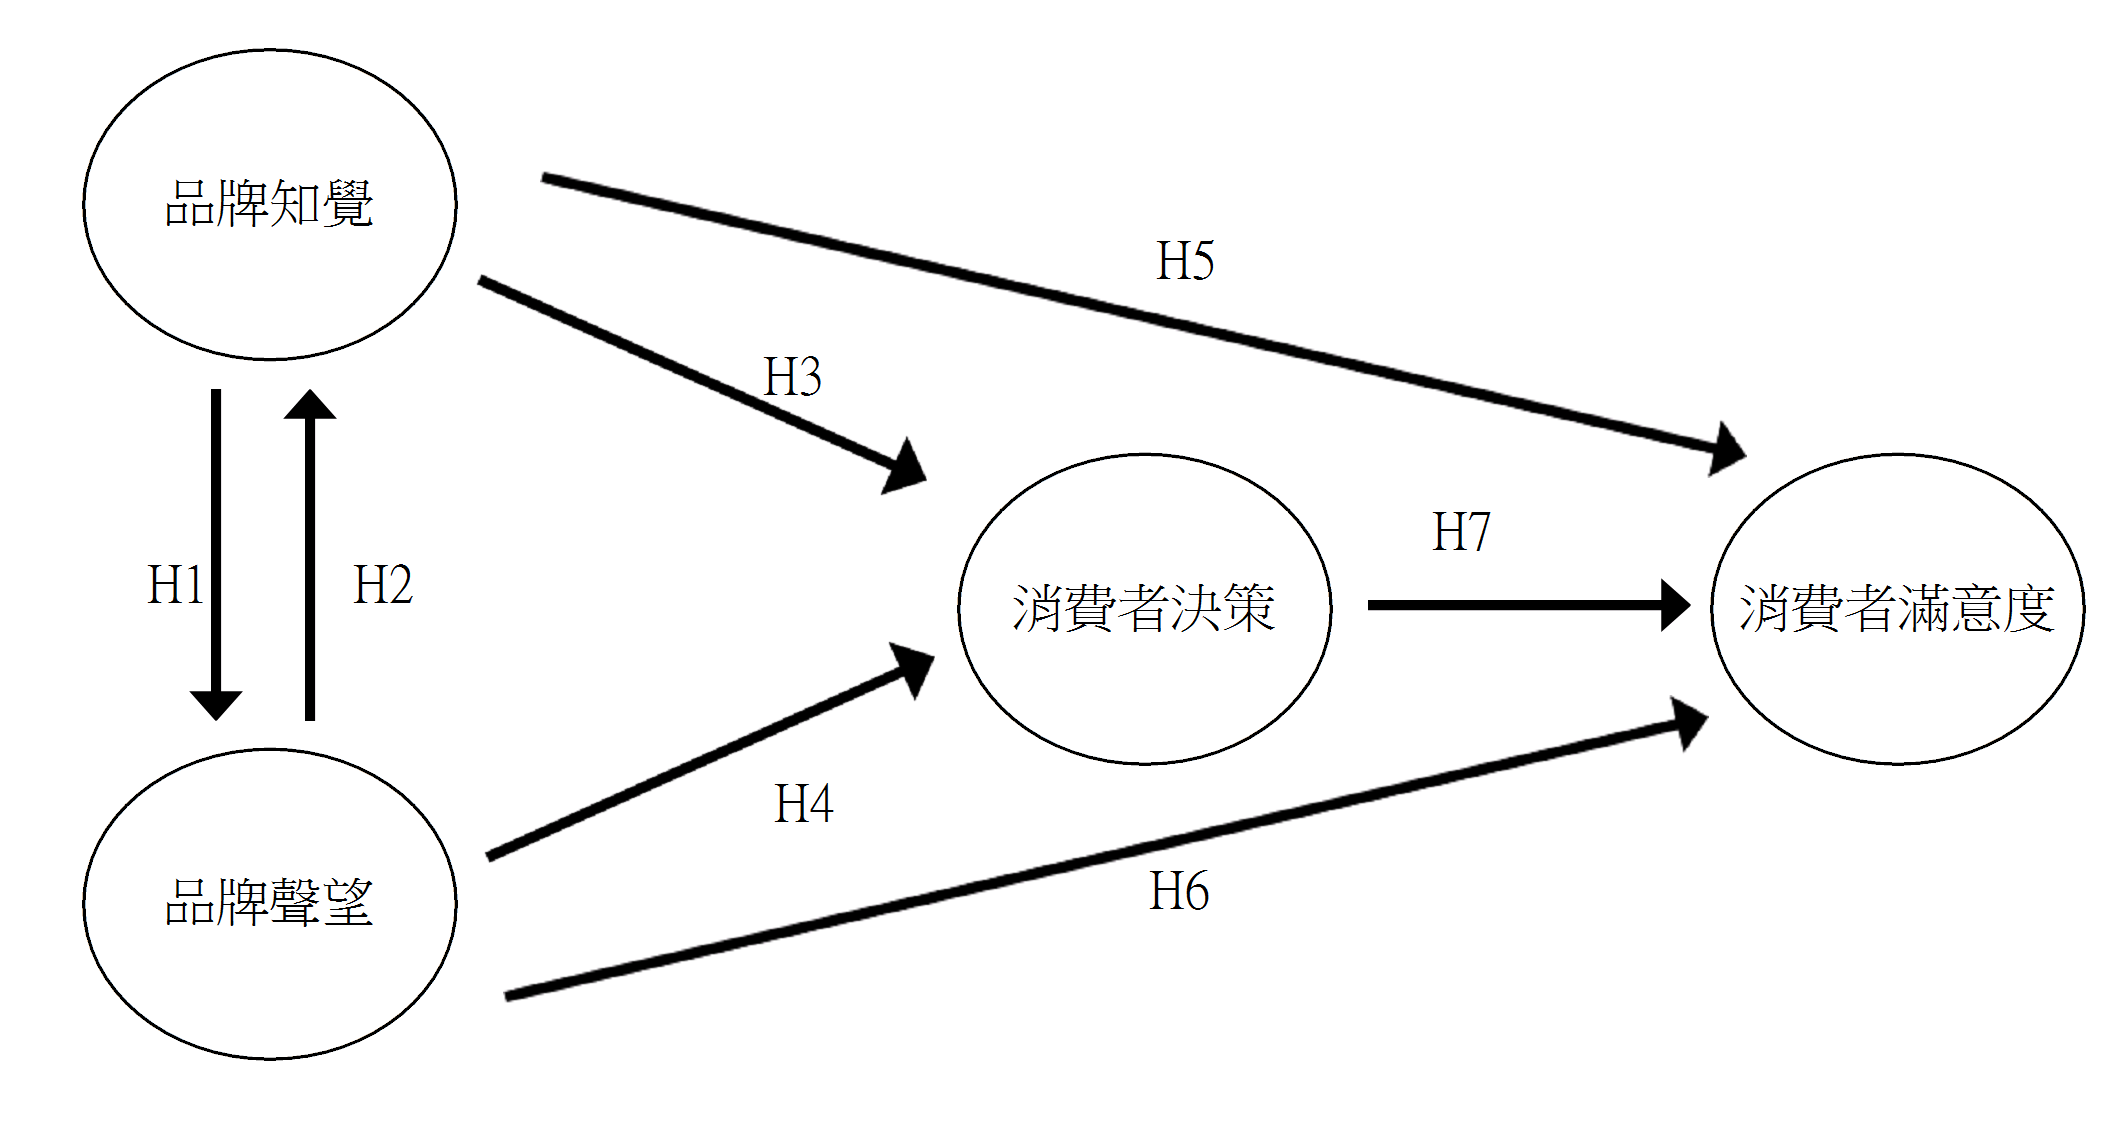
\includegraphics[width=14cm]{images/論文架構.png}
\caption{研究路徑}
\label{fig:ARC}
\end{figure}

在研究路線圖中,因果關係以箭頭符號表示,箭頭所指者為果(依變數),箭頭起使處為因(自變數),以多元迴歸分析而言,符號所指的變項為迴歸方程式的效標變項,箭號起始處則為預測變數。根據本研究中的分析路徑圖,必須進行四個復迴歸分析,如下:

\begin{enumerate}
\item 第一個復迴歸:效標變項為消費者滿意度,預測變項為品牌知覺、品牌聲望、消費者決策。
\item 第二個復迴歸:效標變項為消費者決策,預測變項為品牌知覺、品牌聲望、消費者決策。
\item 第三個復迴歸:效標變項為品牌聲望,預測變項為品牌知覺。
\item 第四個復迴歸:效標變項為品牌知覺,預測變項為品牌聲望。
\end{enumerate}

在完成分析後,如表:\ref{tab:q1},此四條迴歸式之F值皆顯著,第一條迴歸式中,唯有品牌聲望與消費者滿意度具有顯著關係;第二條迴歸式亦只有品牌聲望與消費者決策有顯著關係;第三條與第四條品牌聲望與品牌知覺兩者間有顯著的關係。根據上述之結果。可看出路徑系數與顯著程度繪製於路徑中,有助於瞭解彼此間關係程度,如圖:\ref{fig:ARB}可知,品牌聲望會直接影響消費者滿意度;品牌知覺透過品牌聲望,進而影響消費者滿意度,消費者決策有受到品牌知覺所影響。





\begin{table}[htb]
\caption{路徑分析(復迴歸)}
\label{tab:q1}
\centering
\renewcommand{\arraystretch}{1.2} % 將表格行間距加大為原來的 1.2 倍
\arrayrulewidth=1pt               % 調整線條粗細為 1pt
\tabcolsep=10pt                   % 調整欄間距為 24pt
\begin{tabular}[t]{lclclclclclclcl}  % 第一欄位使用 sans serif 字族
\hline
 迴歸式&自變數&依變數&路徑系數&t&顯著性&F值\\
\hline
迴歸一 &品牌聲望&消費者&0.915&7.175&0.000*&0.000*\\
          &品牌知覺&滿意度&0.018&0.114&0.910& \\
          &消費者決策&      &-0.044&-.261&0.797& \\
\hline
迴歸二&品牌聲望&消費者&0.155&1.415&0.162&0.000* \\
          &品牌知覺&決策  &0.580&5.289&0.000*& \\
\hline
迴歸三&品牌聲望&品牌知覺&0.480&4.6478&0.00*&0.000* \\
\hline
迴歸四&品牌知覺&品牌聲望&0.480&4.678&0.00*&0.000* \\
\hline
\end{tabular}
\end{table}

\begin{figure}[h]
\centering
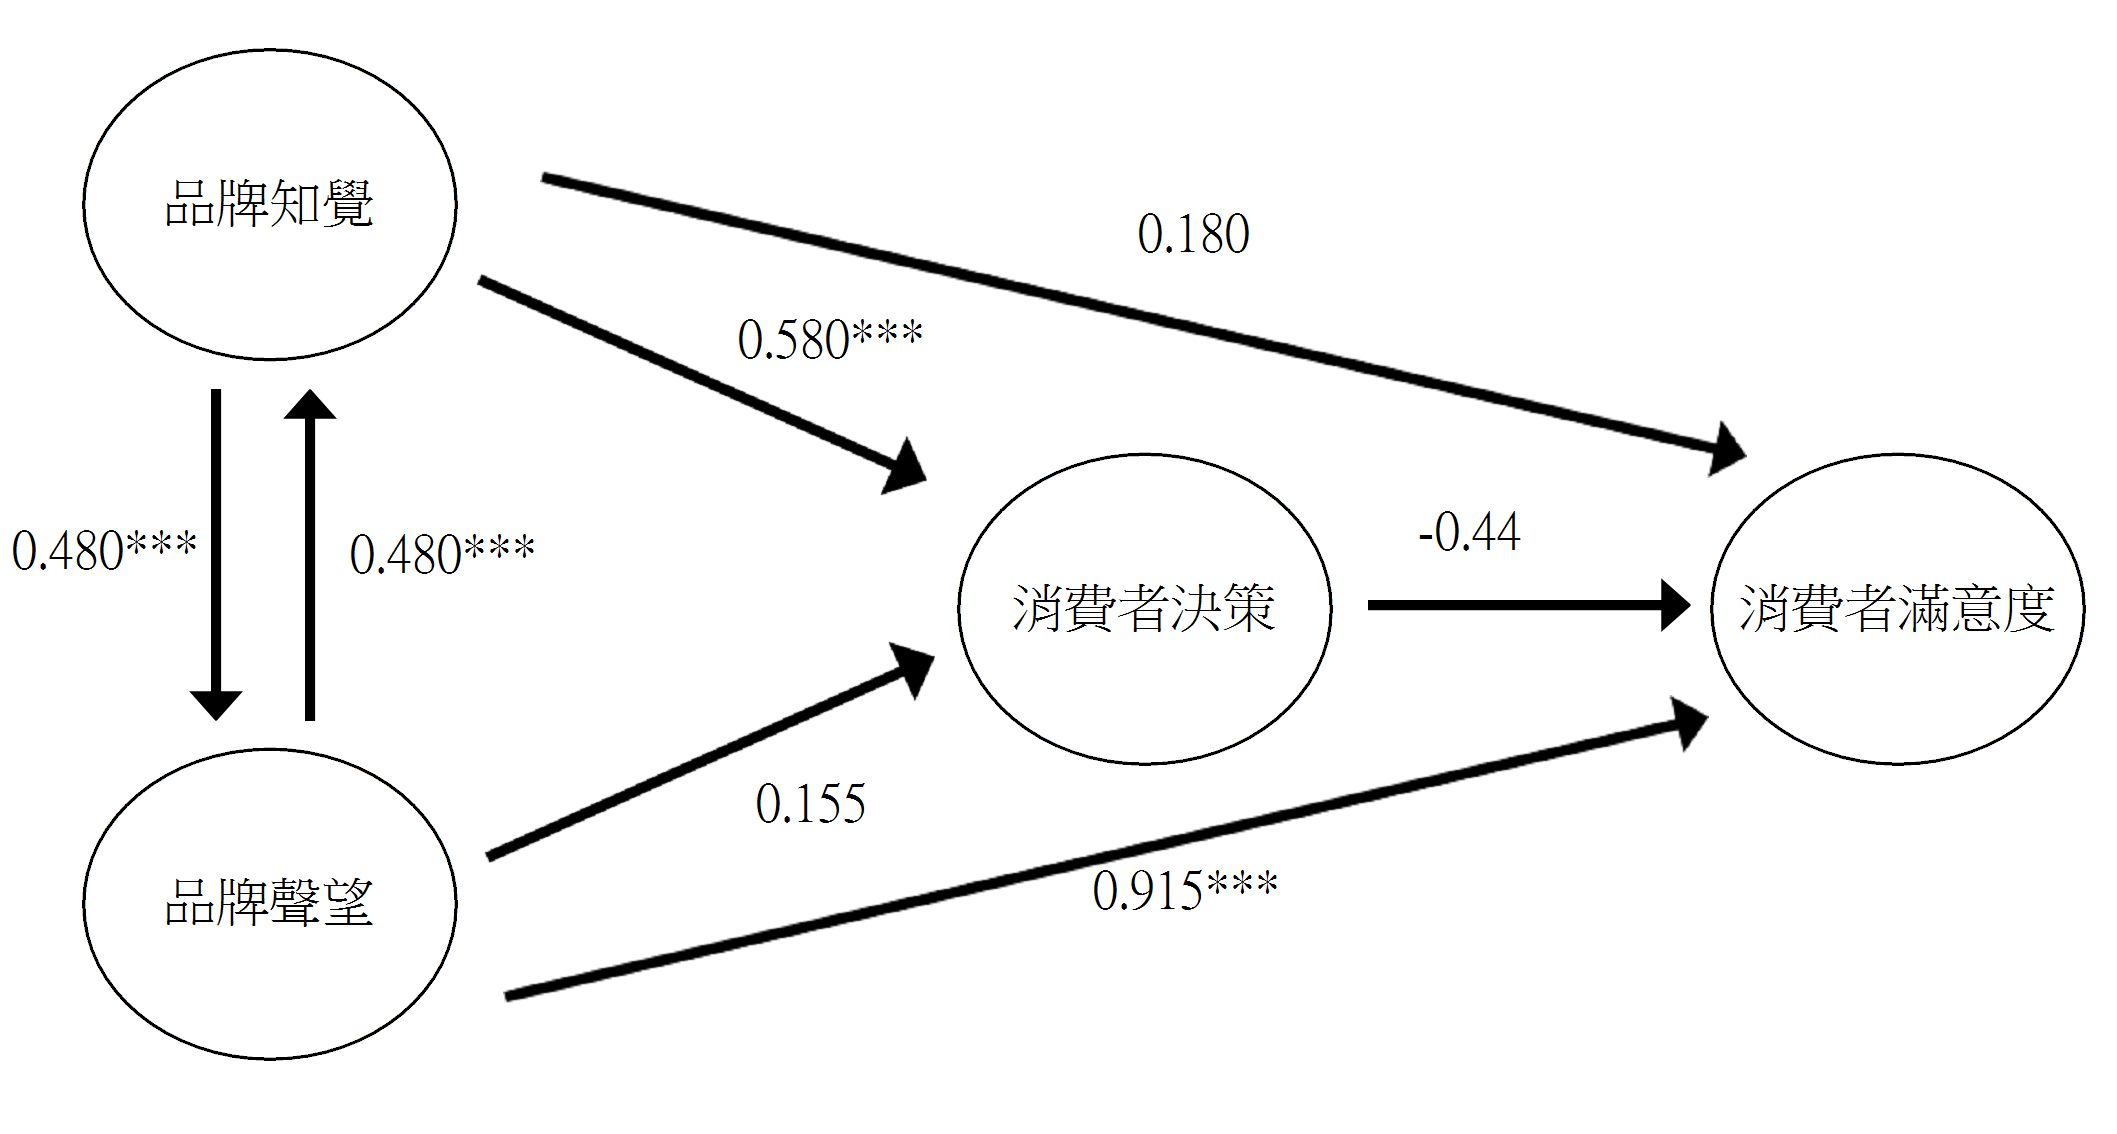
\includegraphics[width=14cm]{images/路徑分析.png}
\caption{研究分析路徑}
\label{fig:ARB}
\end{figure}

\chapter{結論與建議}

\section{結論}
本研究的目的探討品牌知覺,品牌知名度與網路消費者決策和消費者滿意度等變數之間的關係。經發放603份問卷,有效回收問卷599份並使用信度分析與效度分析,描述性統計分析,回歸分析等統計方法來證實分析與研究結果,發現如下:

品牌聲望會影響品牌知覺,同時消費者對於品牌知覺也會影響品牌聲望,因此品牌知覺與品牌聲望會相互影響,而消費者對於品牌知覺與品牌聲望皆會影響消費者決策與影響消費者的滿意度,而消費的決策也會影響消費者滿意度。
\begin{enumerate}
\item 品牌知覺會正向影響品牌聲望有顯著的關係
\item 品牌聲望會正向影響品牌知覺有顯著的關係
\item 品牌知覺會正向影響消費者決策有顯著的關係
\item 品牌聲望會正向影響消費者決策有顯著的關係
\item 品牌知覺會正向影響消費者滿意度有顯著的關係
\item 品牌聲望會正向影響消費者滿意度有顯著的關係
\item 消費者決策會正向影響消費者滿意度有顯著的關係
\end{enumerate}
以上皆成立
因此本研究提出品牌知覺與品牌聲望對公司有所影響,因此品牌聲望與品牌知覺可以有提高整體公司的品牌與獲得消費者滿意度。


\section{未來發展建議}

因此本研究建議企業廠商若要提高顧客滿意度提出了以下建議:
由本研究發現品牌知覺與品牌聲望是相輔相成的正向影響,而且消費者滿意度與影響消費者決策皆會受到聲望與知覺所影響,因此本文提出要有效提升消費者對公司的滿意度可先由品牌知覺做起,就問卷顯示受訪者對品牌知覺主要對商品品質、商品外觀設計感與整體 商品的價值為主要知覺條件,要有效提高品牌知覺要先改 善產品整體價值與服務品質,例如:提升商品故事性與設 計師理念,讓消費者購買到的商品不只是普通商品,而是買到有故事有理念的商品,而達到提高整體商品的價值與 品質而應此提升品牌知覺。
\section{後續研究方向}
\begin{enumerate}
\item 加入不同的觀點去探討:

  由於環境的變遷與時代的進步,由於網路購物成長迅速因此網路購物是個龐大的市場,然而國內對於網路購物之消費者的研究多數仍以滿意度、忠誠度、購買意願為主要的研究目的,是以能夠加入更多不同的觀點來探討。如網路消費行為的決策流程....等

\item 研究角度:

  本研究僅針對消費者角度的個人樣本進行調查與分析,建議後續研究者,可以加入購物網站業者為調查的問卷以便對照樣本,以最此比較購物網站業者與消費者兩者之間對於品牌聲望及品牌知覺的差異為何,使得分析為客觀,更具實用價值。
\end{enumerate}
